\section{Evaluation}
\subsection{Results}
\begin{frame}
Main results,
\begin{itemize}
  \item Spark outperforms Hadoop by up to 20x in iterative machine learning and
  graph applications (speedup mainly comes from avoiding I/O and
  deserialization costs by storing data in memory)
  \item When nodes fail, Spark can recover quickly by rebuilding only the lost
  RDD partitions
  \item able to query 1 TB dataset in 5-7 seconds
\end{itemize}
\end{frame}

\subsection{Methodology}
\begin{frame}
\begin{itemize}
  \item Comparing Spark with Hadoop
	\begin{enumerate}
	  \item Iterative machine learning algorithms: logistic regression, k-means
	  \item PageRank
	\end{enumerate}
  \item Fault recovery
  \item Behavior with insufficient RAM
  \item Scalability
\end{itemize}
\end{frame}

\subsection{Failure Recovery}
\begin{frame}
\begin{figure}
\centering
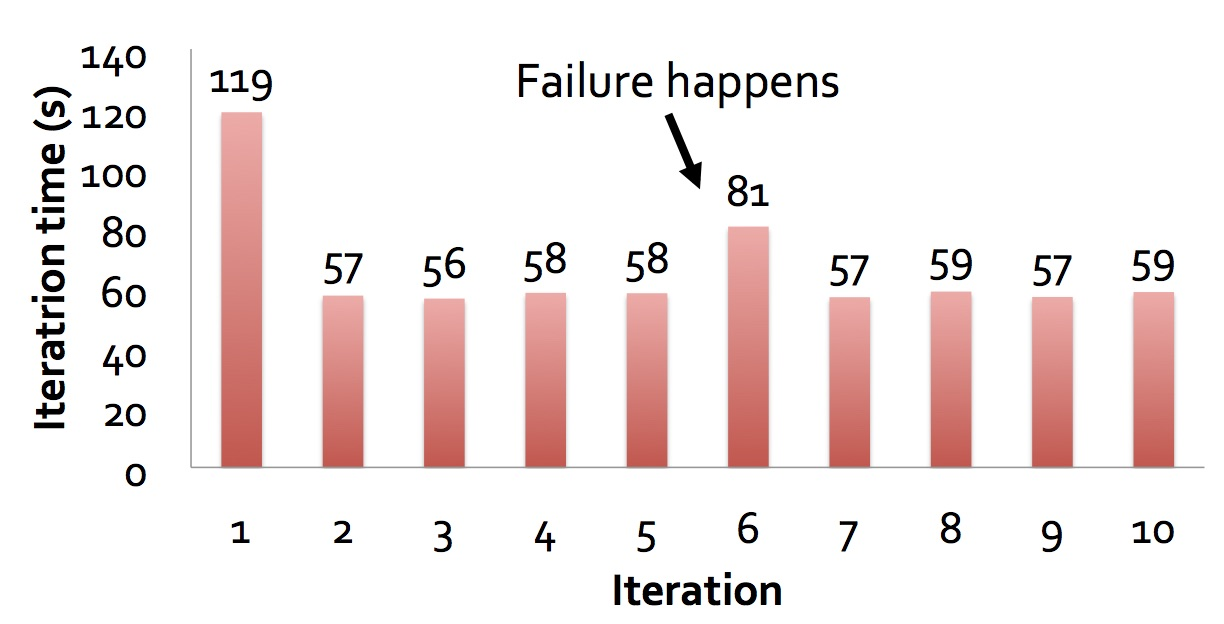
\includegraphics[width=0.80\linewidth]{figures/results-failure-recovery.jpg}
\caption{Failure Recovery [2].}
\end{figure}
\end{frame}

\subsection{Behavior with Insufficient RAM}
\begin{frame}
\begin{figure}
\centering
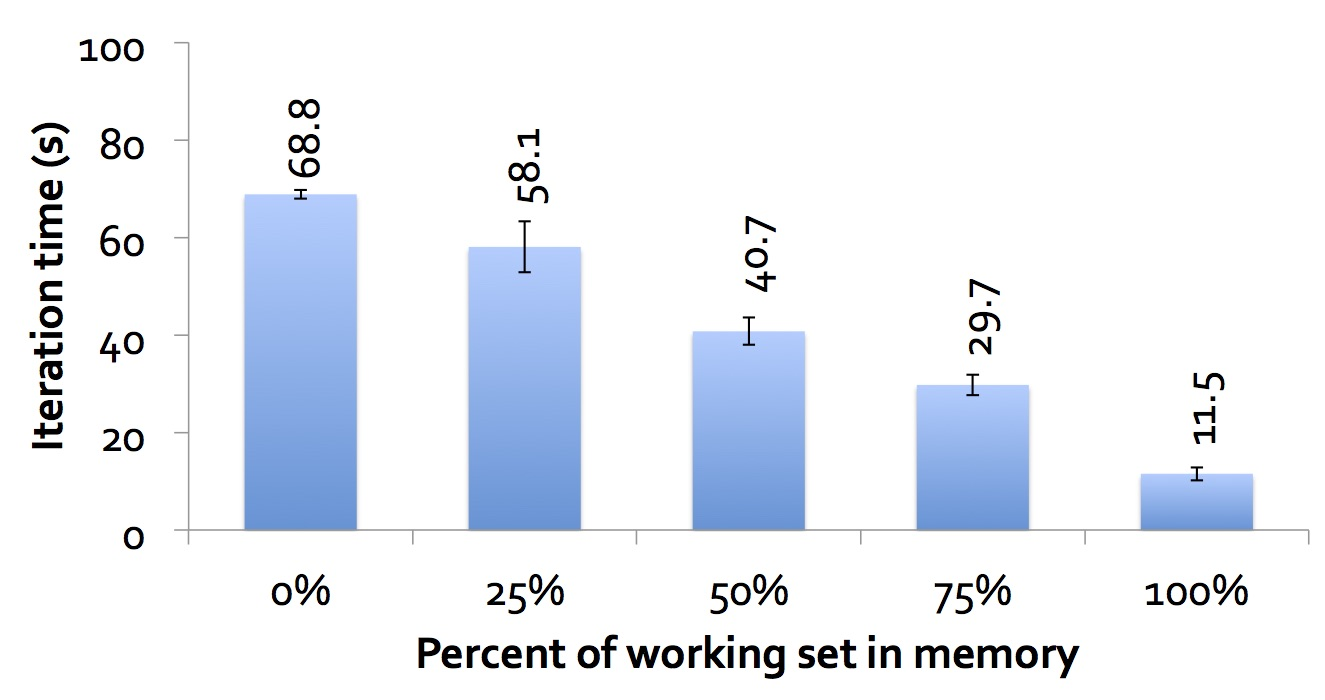
\includegraphics[width=0.80\linewidth]{figures/result-insufficient-ram.jpg}
\caption{Behavior with Insufficient RAM [2].}
\end{figure}
\end{frame}

\subsection{Scalability}
\begin{frame}
\begin{figure}
\centering
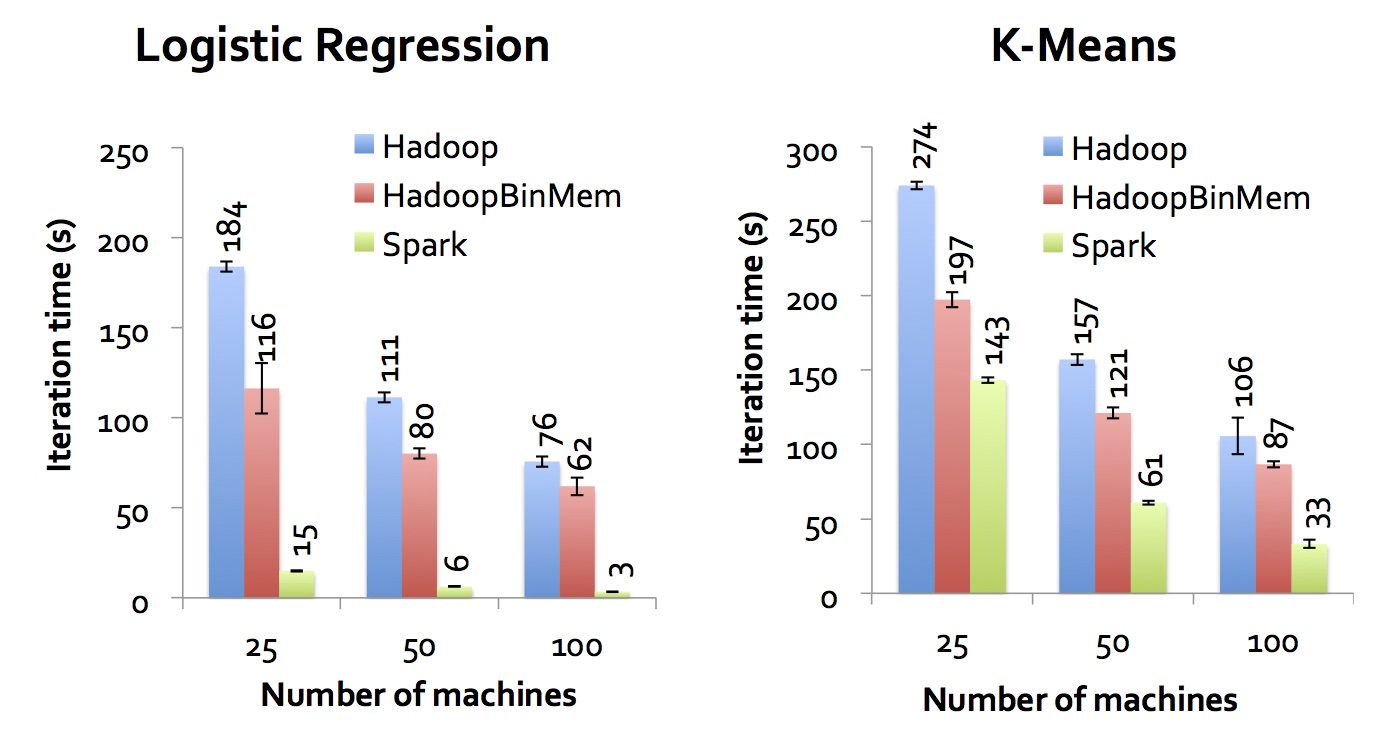
\includegraphics[width=0.80\linewidth]{figures/results-scalability.jpg}
\caption{Scalability [2].}
\end{figure}
\end{frame}
